\documentclass{article}
\usepackage{adjustbox}
\usepackage{float}
\usepackage{textcomp}
\usepackage{graphicx}
\graphicspath{{images/}}
\usepackage{booktabs}
\usepackage{color}
\usepackage{verbatim}
\usepackage{listings}
\usepackage{underscore}
\setcounter{secnumdepth}{5}
\usepackage[bookmarks=true]{hyperref}
\author{Roberto Clapis (841859), Erica Stella (854443)} 
\date{\today}
\title{Politecnico di Milano
	\\A.A. 2015\@-\@2016
	\\Software Engineering 2: ``myTaxiService''
	\\\textbf{P}roject \textbf{P}lan}
\hypersetup{pdftitle={Project Plan},    % title
	pdfauthor={Roberto Clapis, Erica Stella},                     % author
	pdfsubject={Project Plan},                        % subject of the document
	pdfkeywords={TeX, LaTeX, taxi, PP, SoftwareEngineering2}, % list of keywords
	colorlinks=true,       % false: boxed links; true: colored links
	linkcolor=black,       % color of internal links
	citecolor=blue,       % color of links to bibliography
	filecolor=black,        % color of file links
	urlcolor=purple,        % color of external links
}
\begin{document}
\maketitle
\begin{center}
	
\includegraphics{polimi-logo}
\end{center}
\clearpage
\tableofcontents
\clearpage
\section{Introduction}
This document describes the project plan for myTaxiService application.
It presents an analysis of the expected size and effort required 
for the implementation phase calculated respectively with the Function
Points and COCOMO. Then it presents the available resources and how 
they will be allocated to the project tasks and, in the end, it
discusses the possible risks this project might encounter and the
associated recovery actions.
\section{Size and Effort Estimation}
\subsection{Size Estimation - Function Points}
Following Albrecht's method, our application's function points
will be divided in 5 types:
\begin{itemize}
	\item Internal Logical File (ILF): homogeneous set of data used
	and managed by the application.
	\item External Interface File (EIF): homogeneous set of data 
	used by the application but generated and maintained by other.
	\item External Input: elementary operation to elaborate data
	coming from the external environment.
	\item External Output: elementary operation that generates data
	for the external environment.
	\item External Inquiry: elementary operation that involves
	input and output.
\end{itemize}
The function points' types stated above will be weighted as 
specified in the following table.
\begin{center}
	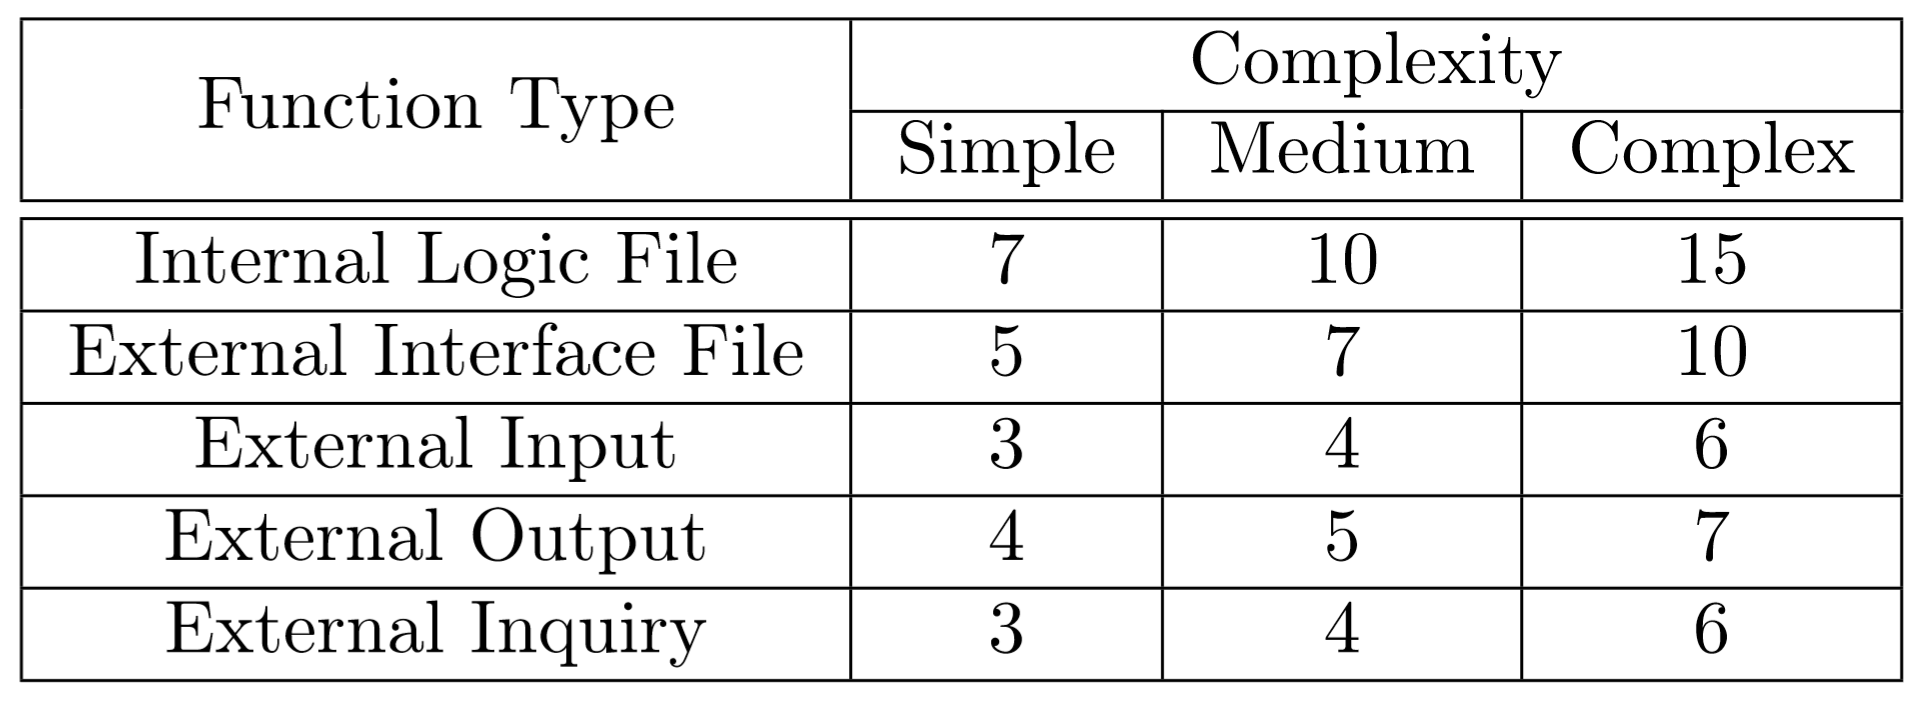
\includegraphics[width = 0.8\textwidth]{FP}
\end{center}
\subsubsection{Internal Logical File}
%TODO
The application stores information about: 
\begin{itemize}
	\item Admins (username, password hash, email)
	\item Users (username, password hash, email)
	\item City zones (nearest zones)
	\item Taxi drivers (taxi code, username, password hash, current zone, availability time)
\end{itemize}
The first three entities have a simple structure as they are composed 
of a small number of fields, while the taxi drivers have a more complex
structure that also needs to be updated frequently. Thus we decide to 
adopt the simple weight for the first three entities and the medium weight
for the last one.
3\texttimes7+1\texttimes10 = 31 FPs concerning ILFs.
\subsubsection{External Interface File}
There are no such things in our project.
\subsubsection{External Input}
\begin{table}[H]
\begin{adjustbox}{width=1.2\textwidth}
\begin{tabular}{*{4}{c}}
\toprule
Function & Complexity & FP computation & FP \\
\midrule
%TODO
registrazione & Medium & 4 & 4\\
login & Easy & 3 & 3\\
logout & Easy & 3 & 3\\
request a taxi & Medium & 4 & 4\\
reserve a taxi & Medium & 4 & 4\\
modify personal data & Medium & 4 & 4\\
toggle taxi driver state & Medium & 4 & 4\\
accept/refuse req and res & Medium x 4 & 4 x 4 &  16\\
location of the taxi driver based on the gps & Medium & 4 & 4\\
add a new taxi driver into the system & Easy & 3 & \\
remove a taxi driver from the system & Easy & 3 & 3 \\
modify taxi drivers' credentials data & Easy & 3 & 3 \\
cancel req/res & Medium x 2 & 4 x 2 & 8 \\
\midrule
&&&\colsum{}\\
\bottomrule
\end{table}
\subsubsection{External Output}
%TODO
suggestion di completamento vie
notifica taxi code del taxi che sta arrivando
notify a request to the taxi driver
notify a reservation

calculate and show ETA - involves calculate the queues and eventually calculate the CAT
\subsubsection{External Inquiry}
%TODO
select a currently active req or res
select a taxi driver for the admin
show the list of taxi drivers for the admin
show all active req and res of a user
list all users of a type
\subsection{Effort Estimation - COCOMO}
%TODO
To convert the function points in SLOC we use a 
conversion factor of 46, as specified here 
http://www.qsm.com/resources/function-point-languages-table
for J2EE.
\begin{center}
	SLOC = FP \texttimes 46 = \texttimes 46 = %TODO
\end{center}
We consider our project with all nominal Cost Drivers and
Scale Drivers so we have an EAF of 1.00 and an
exponent E of 1.0997.
\begin{center}
	€ffort = 2.94 \texttimes EAF \texttimes (KSLOC)
\end{center}
\section{Resource Allocation}
%TODO descrizione
\subsection{Tasks}
RASD:
\begin{itemize}
\item Domain assumptions
\item Functional requirements
\item Non functional requirements
\item Use cases and scenarios
\item User interface
\item Alloy
\end{itemize}
Design Document:
\begin{itemize}
\item
\end{itemize}
Code Inspection:
\begin{itemize}
\item
\end{itemize}
Integration Test Plan Document:
\begin{itemize}
\item 
\end{itemize}
\section{Risks}
\end{document}
